% Tarea 1 - INF-221 Algoritmos y Complejidad - 2026-2
% Benjamin Lira - Rol: 202473586-1

% babel en español rotula las tablas como "Cuadro"; se unifica con el "Tabla"
% que usa \Crefname en la plantilla.
\renewcommand{\tablename}{Tabla}

Las figuras de esta sección fueron generadas por
\verb|code/sorting/scripts/plot_generator.py| y
\verb|code/matrix_multiplication/scripts/plot_generator.py| a partir de los CSV
que producen los programas de medición, y están en
\verb|code/sorting/data/plots/| y \verb|code/matrix_multiplication/data/plots/|.

\subsection{Ordenamiento}

La \Cref{fig:orden-tiempo} muestra el tiempo frente al tamaño de la entrada, en
escala logarítmica en ambos ejes. Esa escala se eligió porque una complejidad
$n^k$ aparece en ella como una recta de pendiente $k$: basta comparar la
inclinación de cada curva con las guías de referencia para leer el exponente. En
los seis paneles las cuatro curvas corren paralelas a la guía de $n \log n$ y
claramente menos inclinadas que la de $n^2$.

\begin{figure}[ht]
  \centering
  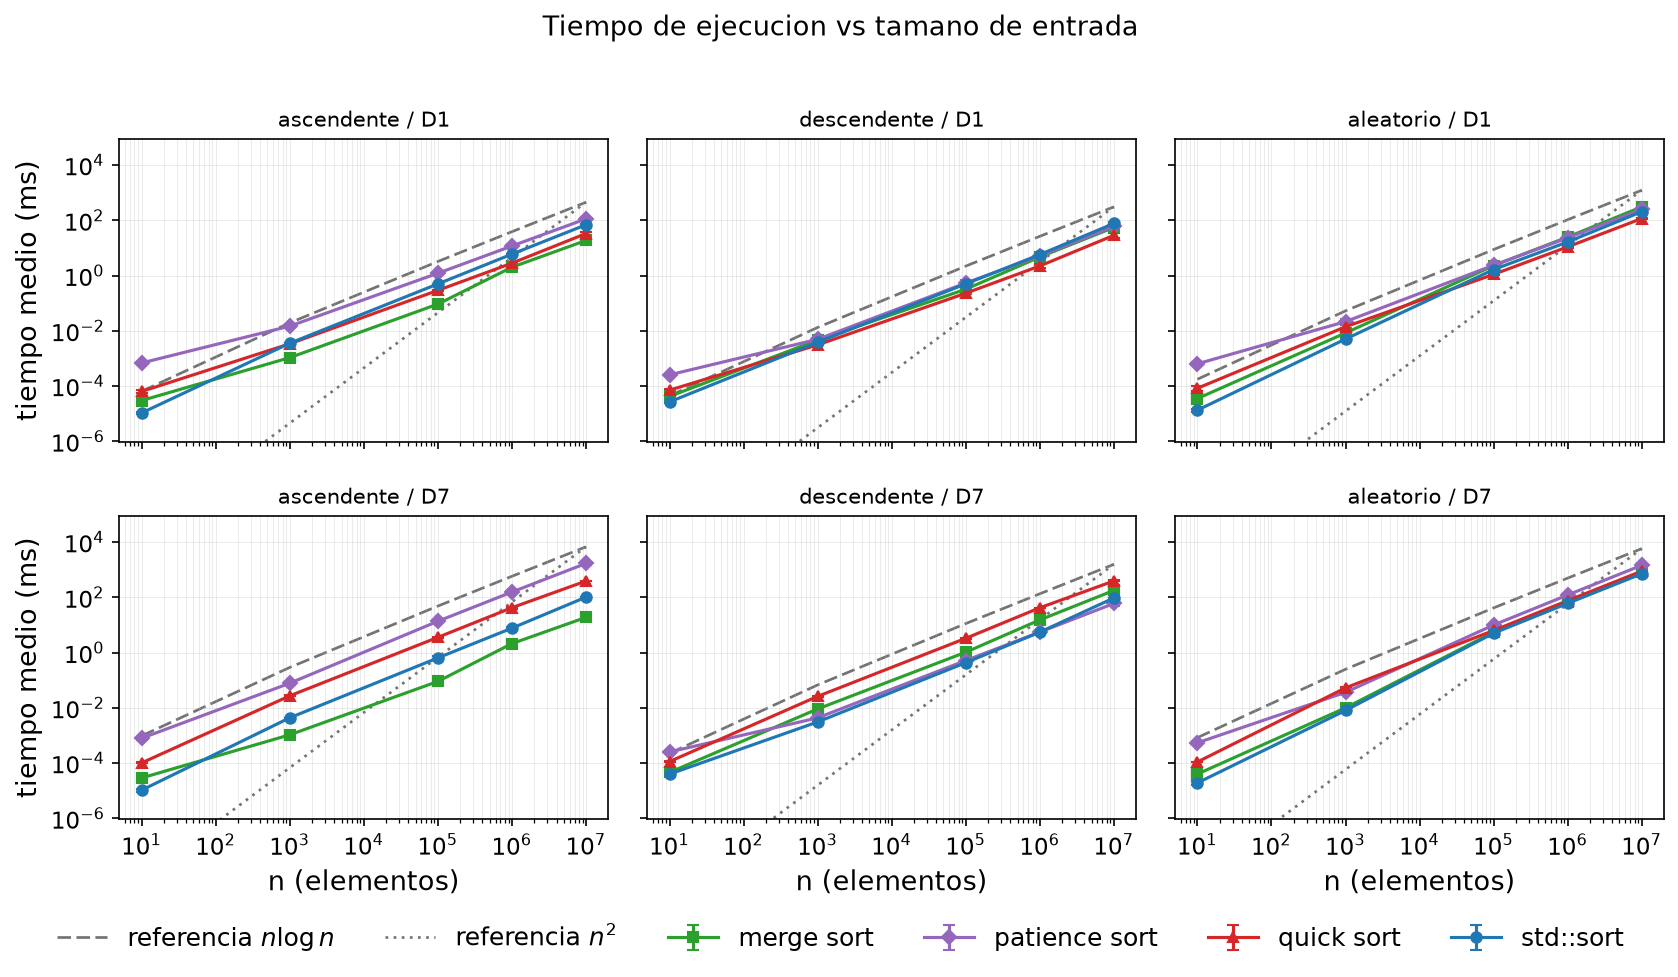
\includegraphics[width=\textwidth]{../code/sorting/data/plots/sorting_tiempo_vs_n.png}
  \caption{Tiempo de ejecución de los cuatro algoritmos de ordenamiento. Cada
  panel es una combinación de tipo de entrada y dominio. Las líneas grises son
  referencias de pendiente, no datos.}
  \label{fig:orden-tiempo}
\end{figure}

La \Cref{tab:orden-exp} cuantifica esa lectura. Ajustando por mínimos cuadrados
$\log t$ contra $\log n$ en el rango $n \geq 10^5$, los veinticuatro exponentes
quedan entre 0,98 y 1,17, frente al 1,07 que predice $n \log n$ en ese rango.
Ninguno se acerca a 1,5 ni a 2: la complejidad teórica describe correctamente el
orden de crecimiento de las cuatro implementaciones sobre las seis familias de
entrada.

\begin{table}[H]
  \centering
  \begin{tabular}{llcccc}
  \hline
  Tipo & Dominio & \texttt{std::sort} & merge sort & quick sort & patience sort \\
  \hline
  ascendente  & D1 & 1,07 & 1,15 & 1,03 & 0,98 \\
  ascendente  & D7 & 1,10 & 1,16 & 1,02 & 1,05 \\
  descendente & D1 & 1,09 & 1,12 & 1,05 & 1,03 \\
  descendente & D7 & 1,17 & 1,12 & 1,04 & 1,03 \\
  aleatorio   & D1 & 1,05 & 1,06 & 1,01 & 1,01 \\
  aleatorio   & D7 & 1,08 & 1,09 & 1,08 & 1,08 \\
  \hline
  \end{tabular}
  \caption{Exponente empírico $k$ por ajuste log-log en $n \geq 10^5$. Para
  $n \log n$ el valor esperado en ese rango es 1,07.}
  \label{tab:orden-exp}
\end{table}

Compartir clase de complejidad no los hace intercambiables. La
\Cref{tab:orden-tiempo} recoge los tiempos en $n = 10^7$: el valor más alto
(1693,3 ms) es 91 veces el más bajo (18,6 ms), y sobre una misma entrada
---ascendente $D7$--- merge sort tarda 18,9 ms y patience sort 1693,3 ms, un
factor de 90.

\begin{table}[H]
  \centering
  \begin{tabular}{llcccc}
  \hline
  Tipo & Dominio & \texttt{std::sort} & merge sort & quick sort & patience sort \\
  \hline
  ascendente  & D1 &   69,0 &   18,6 &   33,2 &  112,8 \\
  ascendente  & D7 &  101,9 &   18,9 &  389,9 & 1693,3 \\
  descendente & D1 &   76,8 &   55,1 &   28,6 &   60,4 \\
  descendente & D7 &   95,1 &  177,9 &  393,1 &   60,1 \\
  aleatorio   & D1 &  205,6 &  306,6 &  116,2 &  249,1 \\
  aleatorio   & D7 &  716,7 &  824,8 &  893,2 & 1453,6 \\
  \hline
  \end{tabular}
  \caption{Tiempo medio en milisegundos para $n = 10^7$, promediado sobre tres
  muestras y tres repeticiones.}
  \label{tab:orden-tiempo}
\end{table}

Cada ventaja tiene un mecanismo identificable. Merge sort gana en las entradas
ascendentes porque omite la mezcla cuando las dos mitades ya están en orden, lo
que reduce ese caso a un recorrido lineal; el mecanismo no depende de los
valores, y en efecto tarda casi lo mismo en $D1$ (18,6 ms) que en $D7$
(18,9 ms). Quick sort es el más rápido en aleatorio $D1$ (116,2 ms) y en
descendente $D1$ (28,6 ms) gracias a su partición de tres vías, que agrupa los
elementos iguales al pivote y no vuelve a tocarlos: con sólo diez valores
distintos el costo pasa a depender del número de valores y no del tamaño, y por
eso el mismo algoritmo sobre la misma forma de entrada resulta entre 8 y 14
veces más rápido en $D1$ que en $D7$. La excepción es ascendente $D1$, donde
merge sort (18,6 ms) le gana con el atajo del párrafo anterior. Patience sort
gana en descendente $D7$ (60,1 ms) porque ahí forma una sola pila, y pierde en
ascendente $D7$ (1693,3 ms) porque forma una por elemento; el número de pilas
$k$ es la longitud de la subsecuencia creciente más larga de la entrada
\cite{aldous1999}, y de él depende todo su costo.

Conviene precisar qué versión de patience sort se midió, porque el
procedimiento tal como se describe originalmente \cite{mallows1963} no fija cómo
buscar la pila destino ni cómo extraer el mínimo, y de esas dos decisiones
depende su clase de complejidad. La transcripción directa recorre las $k$ pilas
para cada uno de los $n$ elementos en ambas fases, lo que da $O(n \cdot k)$ y,
sobre entrada ascendente ---donde $k = n$---, degenera a $\Theta(n^2)$: a
$n = 10^7$ serían unas $10^{14}$ operaciones, fuera del alcance del experimento.
Nuestra implementación aprovecha que los topes de las pilas quedan siempre
ordenados de forma creciente, de modo que la regla «la pila más a la izquierda
cuyo tope sea $\geq x$» es exactamente una búsqueda binaria; y reemplaza el
recorrido de la fase 2 por un montículo de mínimos sobre los topes
\cite{chandramouli2014}. El costo baja a $O(n \log k)$. Ninguna de las dos
sustituciones altera las pilas que se forman ni el orden en que se vacían ---son
decisiones de estructura de datos, no del algoritmo---, y el comportamiento
medido sigue estando gobernado por $k$: los exponentes empíricos de patience
sort quedaron entre 0,98 y 1,08, y entre $n = 10^6$ y $n = 10^7$ el tiempo se
multiplicó por 9,6 a 11,9, frente al factor 100 que implicaría $\Theta(n^2)$.

Esto es lo que hace comparable el experimento de ordenamiento: los cuatro
algoritmos medidos pertenecen a la misma clase de complejidad, de modo que las
diferencias de la \Cref{tab:orden-tiempo} son diferencias de constante y de
sensibilidad a la estructura de la entrada, que es justamente lo que la tarea se
propone medir. Un patience sort $\Theta(n^2)$ habría perdido todas las entradas
grandes por una razón trivial ---pertenecer a otra clase--- y no habría aportado
nada sobre las tres restantes. La contrapartida, que conviene dejar explícita, es
que lo medido bajo el nombre «patience sort» no es la transcripción literal del
procedimiento de \textcite{mallows1963} sino su versión con búsqueda binaria y
montículo; la misma advertencia vale para quick sort, donde se midió la variante
con pivote aleatorio y no la de pivote fijo. El
\texttt{std::sort} de la biblioteca estándar no gana ninguna entrada con
estructura explotable, pero gana la única que no la tiene (aleatorio $D7$,
716,7 ms) y nunca queda más de 5,4 veces por encima del mejor.

En memoria (\Cref{tab:orden-memoria}) la separación es cualitativa y no de grado.
\texttt{std::sort} y quick sort ordenan in situ y no reservan nada. Merge sort
reserva exactamente 38 MB en las seis entradas ---los $10^7$ enteros de su
arreglo auxiliar---, sin depender de los datos. Patience sort varía entre 42 MB y
457 MB para el mismo $n$, un factor de 11 gobernado otra vez por el número de
pilas. La memoria distingue a los algoritmos justo donde el tiempo no lo hace:
los cuatro son $\Theta(n \log n)$, pero dos son $\Theta(1)$ en memoria adicional
y dos son $\Theta(n)$.

\begin{table}[ht]
  \centering
  \begin{tabular}{llcccc}
  \hline
  Tipo & Dominio & \texttt{std::sort} & merge sort & quick sort & patience sort \\
  \hline
  ascendente  & D1 & 0 & 38 & 0 &  42 \\
  ascendente  & D7 & 0 & 38 & 0 & 457 \\
  descendente & D1 & 0 & 38 & 0 &  96 \\
  descendente & D7 & 0 & 38 & 0 &  96 \\
  aleatorio   & D1 & 0 & 38 & 0 &  42 \\
  aleatorio   & D7 & 0 & 38 & 0 &  60 \\
  \hline
  \end{tabular}
  \caption{Memoria adicional solicitada al \emph{heap} en $n = 10^7$, en MB.}
  \label{tab:orden-memoria}
\end{table}

\subsection{Multiplicación de matrices}

Lo más visible en la \Cref{fig:matriz-tiempo} es el punto de cruce: Strassen es
más lento que el algoritmo clásico en $n = 64$ y $n = 256$ (razones 0,57 y 0,64)
y más rápido en $n = 1024$ (razón 2,71). Es lo que predice la teoría: Strassen
cambia una de las ocho multiplicaciones de submatrices por sumas
\cite{strassen1969}, lo que mejora el exponente y empeora la constante, de modo
que sólo conviene por encima de cierto tamaño. El experimento sitúa ese tamaño
entre $n = 256$ y $n = 1024$.

Antes de leer esa curva hay que precisar qué algoritmo se mide en cada punto,
porque no es el mismo en todo el rango. Nuestra implementación de Strassen no
recursiona hasta matrices de $1 \times 1$: por debajo de $32 \times 32$ delega en
el algoritmo clásico, que es la práctica habitual \cite{higham2002} porque la
recursión hasta el escalar pagaría 18 sumas de matrices y varias reservas de
memoria por cada multiplicación. Ese umbral fija cuántos niveles de recursión de
Strassen llega a ejecutar cada tamaño del enunciado:

\begin{center}
\begin{tabular}{ll}
\hline
$n = 16$   & 0 niveles: la llamada cae directo en el caso base \\
$n = 64$   & 1 nivel \\
$n = 256$  & 3 niveles \\
$n = 1024$ & 5 niveles \\
\hline
\end{tabular}
\end{center}

De ahí la forma de las curvas. En $n = 16$ los dos algoritmos no dan tiempos
parecidos sino \emph{idénticos} (0,002 ms ambos, razón 1,00) porque se ejecuta
exactamente el mismo código: lo que la \Cref{tab:matriz} rotula «Strassen» en esa
fila es el algoritmo clásico. A partir de $n = 64$ empieza a ejecutarse Strassen
de verdad y su tiempo se despega \emph{por encima} del clásico ---0,205 ms contra
0,116---, porque a ese tamaño el sobrecosto de las 18 sumas y de las submatrices
temporales pesa más que la multiplicación que se ahorra. Sólo en $n = 1024$, con
cinco niveles activos, el exponente menor alcanza a compensar la constante mayor
y Strassen pasa a ser el más rápido. La consecuencia metodológica es que el punto
de cruce medido no es una propiedad de Strassen en abstracto sino de esta
implementación con umbral 32: subirlo desplaza el cruce hacia $n$ mayores y
bajarlo lo desplaza hacia $n$ menores.

\begin{figure}[ht]
  \centering
  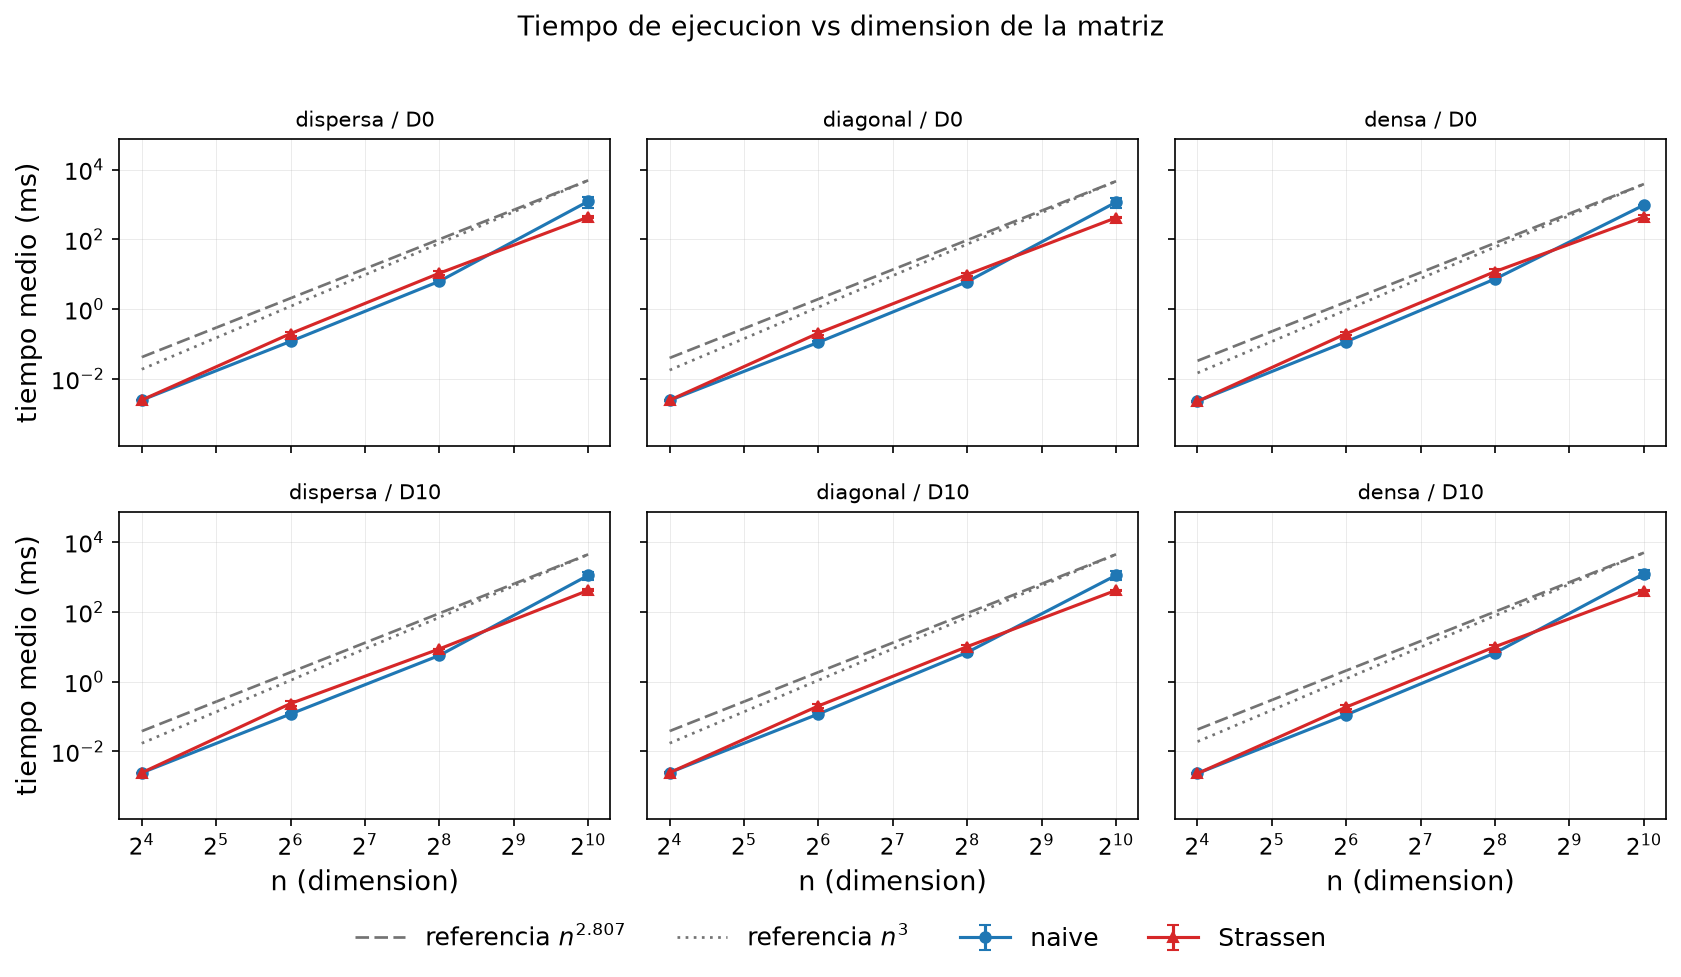
\includegraphics[width=\textwidth]{../code/matrix_multiplication/data/plots/matrix_tiempo_vs_n.png}
  \caption{Tiempo de ejecución de los dos algoritmos de multiplicación. Las
  curvas se cruzan entre $2^8$ y $2^{10}$.}
  \label{fig:matriz-tiempo}
\end{figure}

La \Cref{fig:matriz-tiempo} deja ver el cruce pero no su magnitud, y conviene
explicar por qué. La escala log-log es la adecuada para leer el exponente
empírico, porque una complejidad $n^k$ aparece en ella como una recta de
pendiente $k$; pero por la misma razón comprime las razones. El eje vertical
abarca casi ocho décadas ---de 0,002 ms a más de $10^4$ ms--- y un factor de
2,71 son $\log_{10} 2{,}71 = 0{,}43$ décadas, es decir alrededor del 6\,\% de la
altura del panel. La diferencia más importante del experimento queda reducida a
un margen apenas visible.

La \Cref{fig:matriz-razon} muestra esa misma magnitud sin comprimir: la razón
entre ambos tiempos, en eje lineal, con la horizontal en 1 separando quién gana.
Ahí se lee de un vistazo lo que la \Cref{tab:matriz} da en números: empate exacto
en $n = 16$ ---donde Strassen \emph{es} el algoritmo clásico---, ventaja del
clásico en $n = 64$ y $n = 256$, cruce entre $2^8$ y $2^{10}$, y ventaja de
Strassen en $n = 1024$ por un factor de entre 2,2 y 3,1 según el tipo de matriz.
Que las seis combinaciones de tipo y dominio se mantengan agrupadas en todo el
recorrido es, además, la confirmación gráfica de que el contenido de las
matrices no influye en el tiempo.

\begin{figure}[ht]
  \centering
  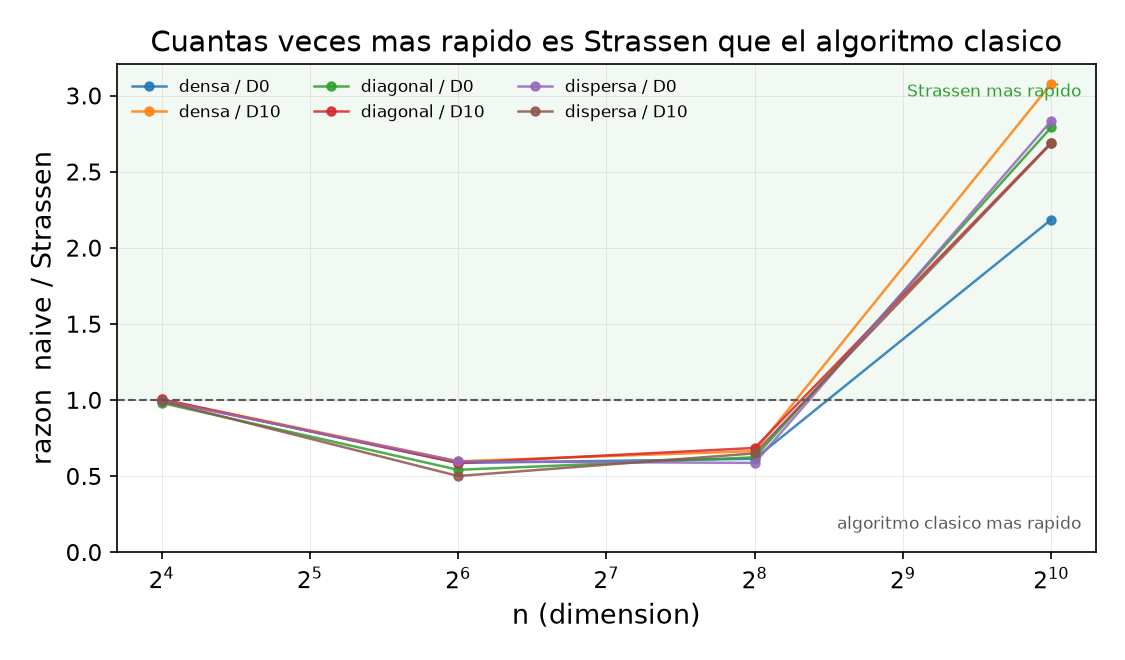
\includegraphics[width=\textwidth]{../code/matrix_multiplication/data/plots/matrix_razon_vs_n.png}
  \caption{Razón entre el tiempo del algoritmo clásico y el de Strassen, en eje
  lineal. Por encima de la horizontal en 1 gana Strassen; por debajo, el clásico.
  Una curva por cada combinación de tipo de matriz y dominio.}
  \label{fig:matriz-razon}
\end{figure}

\begin{table}[H]
  \centering
  \begin{tabular}{crrcccrr}
  \hline
  & \multicolumn{2}{c}{Tiempo (ms)} & &
    \multicolumn{2}{c}{Exponente local $k$} &
    \multicolumn{2}{c}{Memoria (KiB)} \\
  $n$ & naive & Strassen & Razón & naive & Strassen & naive & Strassen \\
  \hline
  16   &    0,002 &   0,002 & 1,00 & --   & --   &    2 &     2 \\
  64   &    0,116 &   0,205 & 0,57 & 2,80 & 3,21 &   35 &   125 \\
  256  &    6,518 &  10,239 & 0,64 & 2,91 & 2,82 &  525 &  1798 \\
  1024 & 1144,681 & 422,918 & 2,71 & 3,73 & 2,68 & 4124 & 23808 \\
  \hline
  \end{tabular}
  \caption{Tiempo medio, razón naive/Strassen, exponente local respecto del
  tamaño anterior, y memoria adicional. Promedios sobre los tres tipos, los dos
  dominios, tres muestras y tres repeticiones.}
  \label{tab:matriz}
\end{table}

El exponente local de la \Cref{tab:matriz} revela algo que un único ajuste
global ocultaría: el algoritmo clásico no crece con exponente constante, sino
que acelera de 2,80 a 2,91 y luego a 3,73, superando su propio $n^3$ teórico en
el último tramo. Strassen hace lo contrario, desacelerando de 3,21 a 2,68. La
explicación es la jerarquía de memoria. El algoritmo clásico recorre la segunda
matriz por columnas, de modo que cada acceso salta una fila completa; mientras
ambas matrices caben en caché el costo es el esperado, pero en $n = 1024$ cada
una ocupa 4 MB, el conjunto de trabajo deja de caber y los fallos de caché se
multiplican. Strassen no sufre la transición porque recursiona hasta submatrices
de $32 \times 32$, que caben siempre.

Esa transición es también la que explica \emph{cuándo} se produjo el cruce, y el
resultado es menos trivial de lo que parece. La teoría predice que la razón entre
ambos tiempos crezca como $n^{3 - \log_2 7} = n^{0{,}193}$, es decir un factor
1,31 cada vez que $n$ se cuadruplica. Entre $n = 64$ y $n = 256$ lo medido se
acerca a eso (factor 1,12). Pero entre $n = 256$ y $n = 1024$ la razón creció por
un factor de 4,25, más del triple de lo previsto. Extrapolando desde $n = 256$
sólo con el exponente asintótico, en $n = 1024$ la razón debería haber sido 0,83
---con Strassen todavía perdiendo--- y el cruce no habría ocurrido hasta
$n \approx 2\,700$, fuera del rango del enunciado. Lo observamos unas ocho veces
antes.

No es que la predicción asintótica falle: es que en ese tramo el algoritmo
clásico dejó de comportarse como $\Theta(n^3)$, y corrió a exponente 3,73 por los
fallos de caché. Las dos observaciones son la misma vista desde dos lados: la
razón creció 4,25 en vez de 1,31 \emph{porque} el denominador teórico dejó de ser
$n^3$. El cruce que reporta la \Cref{fig:matriz-razon} no lo produjo el exponente
de Strassen sino la jerarquía de memoria, que no aparece en ninguna notación
asintótica. Conviene precisar que la extrapolación supone constantes ya estables
en $n = 256$, lo que no es del todo cierto ---Strassen lleva allí sólo tres
niveles de recursión---, de modo que el $n \approx 2\,700$ es un orden de
magnitud y no un valor exacto.

La misma tabla muestra el precio de esa ventaja. El algoritmo clásico sólo
reserva la matriz de salida (4124 KiB en $n = 1024$), mientras que Strassen
reserva 23\,808 KiB, casi seis veces más, porque cada nivel de recursión
construye submatrices temporales y hay cinco niveles activos a la vez. En
$n = 1024$ Strassen es 2,71 veces más rápido y 5,8 veces más caro en memoria.

Por último, el contenido de las matrices no influye en el tiempo: en $n = 1024$
el algoritmo clásico tarda 1111 ms sobre matrices densas, 1147 ms sobre
diagonales y 1176 ms sobre dispersas, una dispersión del 6\,\% comparable al
ruido de medición. Es lo esperado, ya que ejecuta las mismas $n^3$
multiplicaciones aunque la matriz sea casi toda ceros. Contrasta con el problema
de ordenamiento, donde la estructura de la entrada produjo diferencias de dos
órdenes de magnitud.
